\subsection{Линейно независимые циклы}
Опишем два векторных пространства, связанных с графом $G$: пространство циклов и пространство коциклов. Для простоты изложения оба эти пространства задаются над двухэлементным полем $F_2 = \{0, 1\}$, в котором $1 + 1 = 0$ (хотя последующую теорию можно приспособить для произвольного поля). Так, число $e_i$, которое часто встречается в приводимых ниже определениях, равно 0 или 1.

Пусть, как обычно, $G$ — граф с вершинами $v_1, \ldots, v_p$ и рёбрами $x_1, \ldots, x_q$. 0-цепь графа $G$ формально определяется как линейная комбинация $\Sigma e_i v_i$ вершин, а 1-цепь — как линейная комбинация $\Sigma e_i x_i$ рёбер. \textit{Граничный оператор} $\partial$ относит 1-цепи к 0-цепям в соответствии со следующими правилами:
\begin{itemize}
    \item[a)] $\partial$ — линейный оператор;
    \item[б)] если $x = uv$, то $\partial x = u + v$.
\end{itemize}

С другой стороны, \textit{кограничный оператор} $\delta$ относит 0-цепи к 1-цепям в соответствии с правилами:
\begin{itemize}
    \item[a)] $\delta$ — линейный оператор;
    \item[б)] $\delta v = \Sigma e_i x_i$, где $e_i = 1$, если только ребро $x_i$ инцидентно $v$.
\end{itemize}

На рис. 4.6 1-цепь $\sigma_1 = x_1 + x_2 + x_4 + x_9$ имеет «границу»
\[
    \partial \sigma_1 = (v_1 + v_2) + (v_1 + v_3) + (v_2 + v_4) + (v_5 + v_6) = v_3 + v_4 + v_5 + v_6,
\]
а 0-цепь $\sigma_0 = v_3 + v_4 + v_5 + v_6$ имеет «кограницу»
\[
    \delta \sigma_0 = (x_2 + x_4 + x_7) + (x_1 + x_4 + x_9) + (x_5 + x_6 + x_9) + (x_3 + x_7 + x_8) = x_2 + x_3 + x_7 + x_8.
\]

\begin{figure}[h]
    \centering
    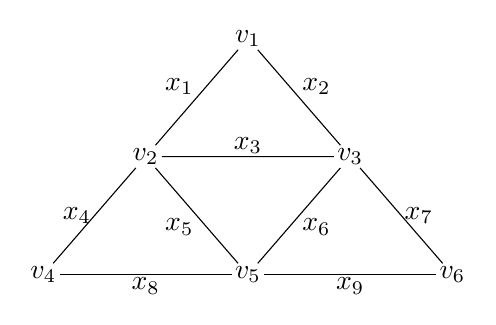
\begin{tikzpicture}[scale=1.5, every node/.style={inner sep=1pt}]
        % Nodes
        \node (v1) at (0, 2) {$v_1$};
        \node (v2) at (-0.866, 1) {$v_2$};
        \node (v3) at (0.866, 1) {$v_3$};
        \node (v4) at (-1.732, 0) {$v_4$};
        \node (v5) at (0, 0) {$v_5$};
        \node (v6) at (1.732, 0) {$v_6$};

        % Edges
        \draw (v1) -- node[above left] {$x_1$} (v2);
        \draw (v1) -- node[above right] {$x_2$} (v3);
        \draw (v2) -- node[above] {$x_3$} (v3);
        \draw (v2) -- node[left] {$x_4$} (v4);
        \draw (v3) -- node[right] {$x_7$} (v6);
        \draw (v4) -- node[below] {$x_8$} (v5);
        \draw (v5) -- node[below] {$x_9$} (v6);
        \draw (v2) -- node[below left] {$x_5$} (v5);
        \draw (v3) -- node[below right] {$x_6$} (v5);
    \end{tikzpicture}

    \caption{Граф для иллюстрации граничного и кограничного операторов.}
\end{figure}

1-цепь с границей 0 называется \textit{циклическим вектором}\footnote{Большинство топологов и некоторые специалисты по теории графов называют это «циклом». В свою очередь вместо нашего понятия простого цикла они используют термины «контуры», «элементарные циклы», «полигоны».} графа $G$. Циклический вектор можно рассматривать как множество простых циклов, не имеющих попарно общих рёбер. Множество всех циклических векторов образует над $F_2$ векторное пространство, называемое \textit{пространством циклов} графа $G$. \textit{Базис циклов} графа $G$ определяется как базис пространства циклов графа $G$, состоящий только из простых циклов. Будем говорить, что циклический вектор $Z$ зависит от простых циклов $Z_1, Z_2, \ldots, Z_k$, если его можно представить в виде $\sum_{i=1}^{k} e_i Z_i$. Таким образом, можно сказать, что базис циклов графа $G$ является максимальным набором независимых простых циклов графа $G$ или минимальным набором простых циклов, от которых зависят все циклы.

Разрез связного графа — это множество рёбер, удаление которых приводит к несвязному графу. Коциклом называется минимальный разрез. Кограницей графа $G$ называется кограница некоторой его 0-цепи. Кограница набора $U$ вершин есть не что иное, как множество всех рёбер, соединяющих вершины из $U'$ с вершинами, не принадлежащими $U'$. Очевидно, что каждая кограница является разрезом. Поскольку коцикл определяется как минимальный разрез графа $G$, а любой минимальный разрез есть кограница, то всякий коцикл является минимальной ненулевой кограницей. Множество всех кограниц графа $G$ называется пространством коциклов графа $G$, а базис этого пространства, состоящий только из коциклов, называется базисом коциклов графа $G$.

Перейдём теперь к построению для пространства циклов графа $G$ базиса, который соответствует остову $T$. В связном графе $G$ хордой остова $T$ называется ребро графа, не принадлежащее $T$. Ясно, что подграф графа $G$, содержащий остов $T$ и его произвольную хорду, имеет только один (простой) цикл. Множество $Z(T)$ всех таких циклов (каждая хорда «порождает» один цикл) независимо, так как каждый из них содержит ребро, не принадлежащее ни одному из остальных циклов. Более того, любой цикл $Z$ зависит от множества $Z(T)$, причём $Z$ есть симметрическая разность циклов, которые определяются хордами остова $T$, принадлежащими $Z$. Поэтому, определяя циклический ранг $m(G)$ как число простых циклов базиса пространства циклов графа $G$, можно сформулировать следующий результат.

\textbf{Теорема 4.5.} Циклический ранг связного графа $G$ равен числу хорд любого остова в $G$.

\textbf{Следствие 4.5 (а).} Если $G$ — связный $(p, q)$-граф, то $m(G) = q - p + 1$.

\textbf{Следствие 4.5 (б).} Если $G$ — это $(p, q)$-граф с $k$ компонентами, то $m(G) = q - p + k$.

\footnote{Остовом называется остовный подграф, являющийся деревом. — Прим. ред.}

Подобные утверждения справедливы также для пространства коциклов.
Кодерево $T^*$ остова $T$ в связанном графе $G$ --- это остовный подграф в $G$, содержащий только те рёбра графа $G$, которые не принадлежат $T$.
Под кодеревом графа $G$ понимается кодерево некоторого остова $T$.
На рис. 4.7 показаны остов $T$ и его кодерево $T^*$ для графа $G$, представленного также на рис. 4.6.

\begin{figure}[h]
    \centering
    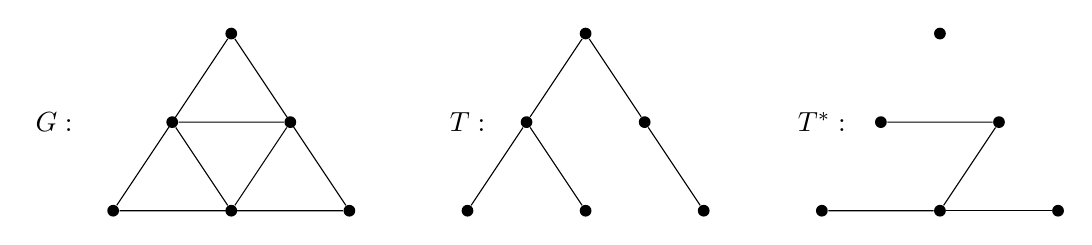
\begin{tikzpicture}[scale=1.5, every node/.style={circle, fill, inner sep=1.5pt}]

        % Graph G
        \node (a) at (0, 1.5) {};
        \node (b) at (-1, 0) {};
        \node (c) at (1, 0) {};
        \node (d) at (0, 0) {};
        \node (e) at (-0.5, 0.75) {};
        \node (f) at (0.5, 0.75) {};

        \draw (a) -- (b) -- (c) -- (a);
        \draw (d) -- (c);
        \draw (e) -- (f);
        \draw (d) -- (e);
        \draw (d) -- (f);

        \node[draw=none, fill=none] at (-1.5, 0.75) {$G:$};

        % Tree T
        \node (g) at (3, 1.5) {};
        \node (h) at (2.5, 0.75) {};
        \node (i) at (3.5, 0.75) {};
        \node (j) at (2, 0) {};
        \node (k) at (3, 0) {};
        \node (l) at (4, 0) {};

        \draw (g) -- (h) -- (j);
        \draw (g) -- (i) -- (l);
        \draw (h) -- (k);

        \node[draw=none, fill=none] at (2, 0.75) {$T:$};

        Co-tree T*
        \node (m) at (6, 1.5) {};
        \node (n) at (5.5, 0.75) {};
        \node (o) at (6.5, 0.75) {};
        \node (p) at (5, 0) {};
        \node (q) at (6, 0) {};
        \node (r) at (7, 0) {};

        \draw (n) -- (o) -- (q) -- (p);
        \draw (q) -- (r);

        \node[draw=none, fill=none] at (5, 0.75) {$T^*:$};
    \end{tikzpicture}
    \caption{Граф, дерево, кодерево}
\end{figure}

Рёбра графа $G$, не принадлежащие $T^*$, назовем ветвями графа $G$ (относительно $T^*$. --- Перев.).
Подграф графа $G$, состоящий из $T^*$ и любой одной ветви, содержит ровно один коцикл.
Множество всех таких коциклов (каждая ветвь <<порождает>>c один коцикл) является базисом пространства коциклов графа $G$.

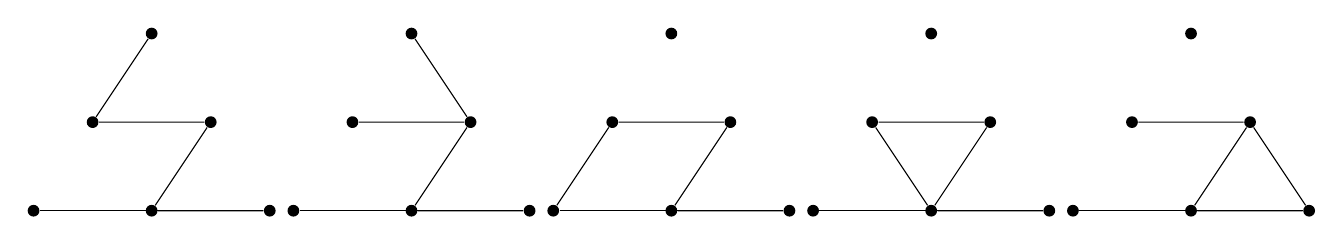
\begin{tikzpicture}[scale=1.5, every node/.style={circle, fill, inner sep=1.5pt}]

    % First graph
    \begin{scope}
    \node (a1) at (0, 1.5) {};
    \node (b1) at (-1, 0) {};
    \node (c1) at (1, 0) {};
    \node (d1) at (0, 0) {};
    \node (e1) at (-0.5, 0.75) {};
    \node (f1) at (0.5, 0.75) {};

    \draw (a1) -- (e1) -- (f1) -- (d1) -- (c1);
    \draw (c1) -- (b1);
    \end{scope}
    % Second graph
    \begin{scope}
        [xshift=2.2cm]
        \node (a) at (0, 1.5) {};
        \node (b) at (-1, 0) {};
        \node (c) at (1, 0) {};
        \node (d) at (0, 0) {};
        \node (e) at (-0.5, 0.75) {};
        \node (f) at (0.5, 0.75) {};
    
        \draw (e) -- (f) -- (d) -- (c);
        \draw (c) -- (b);
        \draw (a) -- (f);
    \end{scope}
    
    % Third graph
    \begin{scope}
        [xshift=4.4cm]
        \node (a) at (0, 1.5) {};
        \node (b) at (-1, 0) {};
        \node (c) at (1, 0) {};
        \node (d) at (0, 0) {};
        \node (e) at (-0.5, 0.75) {};
        \node (f) at (0.5, 0.75) {};
    
        \draw (b) -- (e) -- (f) -- (d) -- (c);
        \draw (c) -- (b);
    \end{scope}
    
    % Fourth graph

    \begin{scope}
        [xshift=6.6cm]
        \node (a) at (0, 1.5) {};
        \node (b) at (-1, 0) {};
        \node (c) at (1, 0) {};
        \node (d) at (0, 0) {};
        \node (e) at (-0.5, 0.75) {};
        \node (f) at (0.5, 0.75) {};
    
        \draw (d) -- (e) -- (f) -- (d) -- (c);
        \draw (c) -- (b);
    \end{scope}
    
    % Fifth graph

    \begin{scope}
        [xshift=8.8cm]
        \node (a) at (0, 1.5) {};
        \node (b) at (-1, 0) {};
        \node (c) at (1, 0) {};
        \node (d) at (0, 0) {};
        \node (e) at (-0.5, 0.75) {};
        \node (f) at (0.5, 0.75) {};
    
        \draw (e) -- (f) -- (d) -- (c) -- (f);
        \draw (c) -- (b);
    \end{scope}
    
    \end{tikzpicture}

На рис. 4.8 для графа $G$ и его кодерева $T^*$ (рис. 4.7) изображены коциклы, образующие пространство коциклов, --- они отмечены жирными линиями. \textit{Коциклический ранг} $t^*(G)$ равен числу коциклов в базисе пространства коциклов графа $G$.

\textbf{Теорема 4.6.} Коциклический ранг связного графа $G$ равен числу рёбер любого его остова.

Как и в случае циклов, немедленно получаем два следствия.

\textbf{Следствие 4.6 (а).} Если $G$ --- связный $(p, q)$-граф, то $t^*(G) = p - 1$.

\textbf{Следствие 4.6 (б).} Если $G$ --- это $(p, q)$-граф с $k$ компонентами, то $t^*(G) = p - k$.

\textbf{Замечание.} Из теоремы 4.5 можно получить частное утверждение (для одномерного случая) одного важного общего результата о симплициальных комплексах. Для каждого симплициального комплекса имеет место уравнение Эйлера — Пуанкаре
\[
a_0 - a_1 + a_2 - \ldots = \beta_0 - \beta_1 + \beta_2 - \ldots,
\]
где $\beta_n$ — числа Бетти, а $a_n$ — количество симплексов соответствующих размерностей. По определению $\beta_n$ является рангом векторного пространства $n$-мерных циклов. Напомним (гл. 1), что любой граф есть симплициальный комплекс, вершины соответствуют 0-симплексам, а ребра соответствуют 1-симплексам. Для графа $G$ имеем $\beta_n = 0$ (число его компонент связности) и $\beta_1 = m(G)$ (число его независимых циклов). Поскольку графы не содержат $n$-симплексов при $n > 1$, то $a_n = \beta_n = 0$ для всех $n \geq 1$. Поэтому $a_0 - a_1 = \beta_0 - \beta_1$, так что $p - q = k - m(G)$ (в следствие 4.5) дает уравнение Эйлера — Пуанкаре для графов.

